\begin{figure}[H]
\centering
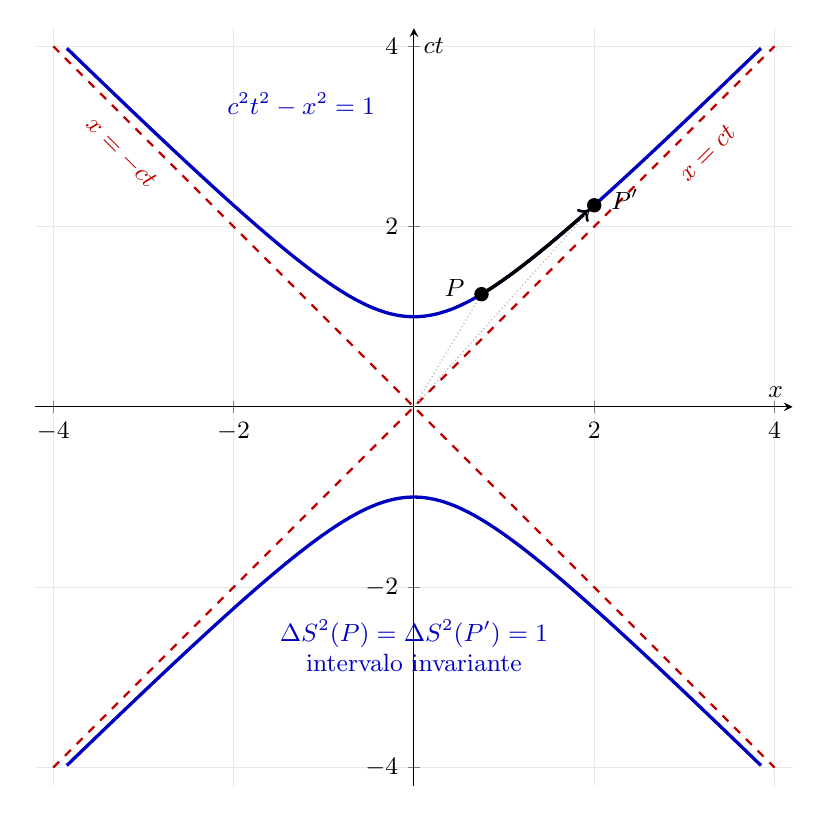
\begin{tikzpicture}
\begin{axis}[
    width=0.94\textwidth,
    height=11.2cm,
    xmin=-4.2,
    xmax=4.2,
    ymin=-4.2,
    ymax=4.2,
    axis lines=middle,
    axis equal image,
    xlabel={$x$},
    ylabel={$ct$},
    xtick={-4,-2,0,2,4},
    ytick={-4,-2,0,2,4},
    grid=major,
    grid style={gray!18},
    tick label style={font=\small},
    label style={font=\small},
    clip=false
]
    \addplot[red!75!black,thick,dashed,domain=-4:4] {x};
    \addplot[red!75!black,thick,dashed,domain=-4:4] {-x};

    \addplot[blue!75!black,very thick,domain=-3.85:3.85,samples=180]
        {sqrt(x^2+1)};
    \addplot[blue!75!black,very thick,domain=-3.85:3.85,samples=180]
        {-sqrt(x^2+1)};

    \addplot[only marks,mark=*,mark size=2.4pt,black]
        coordinates {(0.75,1.25) (2,2.23607)};
    \node[anchor=east,font=\small] at (axis cs:0.67,1.32) {$P$};
    \node[anchor=west,font=\small] at (axis cs:2.08,2.30) {$P'$};

    \addplot[black,very thick,->,domain=0.79:1.94,samples=80]
        {sqrt(x^2+1)};

    \draw[gray!65,densely dotted] (axis cs:0,0) -- (axis cs:0.75,1.25);
    \draw[gray!65,densely dotted] (axis cs:0,0) -- (axis cs:2,2.23607);
    \node[font=\small,blue!75!black,align=center]
        at (axis cs:0,-2.65)
        {$\Delta S^2(P)=\Delta S^2(P')=1$\\
         intervalo invariante};

    \node[blue!75!black,font=\small]
        at (axis cs:-1.25,3.35)
        {$c^2t^2-x^2=1$};
    \node[red!75!black,rotate=45,font=\small]
        at (axis cs:3.25,2.82) {$x=ct$};
    \node[red!75!black,rotate=-45,font=\small]
        at (axis cs:-3.25,2.82) {$x=-ct$};
\end{axis}
\end{tikzpicture}
\caption{Hipérbola de intervalo espacio-temporal constante, $\Delta S^2=c^2t^2-x^2=1$. Una transformación de Lorentz desplaza las coordenadas del evento de $P$ a $P'$ a lo largo de la misma hipérbola, sin modificar el intervalo. Las líneas de luz son sus asíntotas.}
\label{fig:hiperbolas-minkowski}
\end{figure}